\documentclass[a4paper, 12pt]{article}
\usepackage{graphicx}
\usepackage{geometry}
\usepackage{amsmath}
\usepackage{natbib}
\usepackage{hyperref}
\usepackage{booktabs}
\usepackage{listings}
\usepackage{color}

% Geometry settings
\geometry{left=3cm, right=3cm, top=3cm, bottom=3cm}

% Define a style for the listings
\lstset{
  basicstyle=\ttfamily\small,
  breaklines=true,
  breakatwhitespace=true,
  showspaces=false,
  showstringspaces=false,
  numbers=left,
  numberstyle=\tiny,
  stepnumber=1,
  numbersep=5pt,
  tabsize=2,
  captionpos=b,
  frame=single,
  rulecolor=\color{black},
  language=bash,
  morekeywords={cd, cdo, wslpath}
}

% Title Page
\title{Hydrologic Model Setup for Orontes River Basin}
\author{Sepehr Sadeghzadeh Saadat \\ Student Number: 010200912}
\date{\today}

\begin{document}

% Title page with university logo
\begin{titlepage}
    \centering
    
\includegraphics[width=0.8\textwidth]{İstanbul_Teknik_Üniversitesi_Logo.jpg}\par\vspace{1cm}
    {\scshape\LARGE Istanbul Technical University \par}
    \vspace{0.5cm}
    {\scshape\Large Faculty of Civil Engineering \par}
  
    \vspace{1.5cm}
    {\huge\bfseries Hydrologic Model Setup for Orontes River Basin\par}
    \vspace{2cm}
    {\Large\itshape Sepehr Sadeghzadeh Saadat \par}
    {\Large\ Student Number: 010200912 \par}
    \vfill
    Supervised by\par
    Prof. Mehmet Cüneyd Demirel \par
    Research Assistant	Selahattin Utku Yılmaz \par
    \vfill
    Course Code: INS345E (Hydrology) \par
    CNR Code: 21984 \par
    \vfill
    {\large \today\par}
\end{titlepage}

% Abstract
\begin{abstract}
This report describes the setup and calibration of a hydrologic model for the Orontes River Basin at the DEMIRKOEPRUE station (station number 6692100). The model uses river discharge data from the GRDC data portal, meteorological data processed with CDO, and the HBV model implemented in Excel. The performance of the model is evaluated using the Nash-Sutcliffe efficiency.
\end{abstract}

% Table of contents
\tableofcontents
\newpage

\section{Introduction}
In this homework assignment, we applied various hydrological data processing and modeling techniques to set up a hydrologic model for the Orontes River Basin. The steps involved included downloading and processing river discharge and meteorological data, and calibrating the HBV model to simulate river discharge.

\section{Data Acquisition}
\subsection{River Discharge Data}
River discharge data was obtained from the GRDC data portal for station number 6692100 (DEMIRKOEPRUE). The data included the basin border file in GeoJSON format, which was viewed in QGIS to identify the basin's extent.

\subsection{Meteorological Data}
Meteorological data required for the model includes precipitation (P), potential evapotranspiration (PET), and average temperature (T). These were processed using CDO tools to generate the necessary time series for the HBV model.

\section{Hydrologic Modeling}
\subsection{Basin Extent}
The extent of the Orontes River Basin was determined using QGIS, with the following coordinates:
\begin{verbatim}
EPSG:4326 - WGS 84 - Geographic
Extent: 35.9624999999999986,33.7332999999999998: 37.5292000000000030,36.2875000000000014
\end{verbatim}

\subsection{Data Processing with CDO}
The meteorological data was processed using the following CDO commands:

\begin{lstlisting}
wslpath 'C:\ITU\INS 354E\2.Project\2.try'
cd '/mnt/c/ITU/INS 354E/2.Project/2.try'
cdo sellonlatbox,35.75,37.75,33.50,36.50 pre_TR.nc pre_Orontes.nc
cdo sellonlatbox,35.75,37.75,33.50,36.50 pet_TR.nc pet_Orontes.nc
cdo sellonlatbox,35.75,37.75,33.50,36.50 tavg_TR.nc Tavg_Orontes.nc
cdo fldmean pre_Orontes.nc TS_pre_Orontes.nc
cdo fldmean pet_Orontes.nc TS_pet_Orontes.nc
cdo fldmean Tavg_Orontes.nc TS_Tavg_Orontes.nc 
cdo seldate,1975-10-01,1986-09-30 TS_pre_Orontes.nc pre1975_86.nc
cdo seldate,1975-10-01,1986-09-30 TS_pet_Orontes.nc pet1975_86.nc
cdo seldate,1975-10-01,1986-09-30 TS_Tavg_Orontes.nc Tavg1975_86.nc
cdo outputtab,date,value pre1975_86.nc > pre1975_86.csv
cdo outputtab,date,value pet1975_86.nc > pet1975_86.csv
cdo outputtab,date,value Tavg1975_86.nc > Tavg1975_86.csv
\end{lstlisting}

These commands were executed step-by-step to process the meteorological data as follows:

1. \texttt{wslpath 'C:\ITU\INS 354E\2.Project\2.try'}: Converts the Windows file path to a format compatible with WSL (Windows Subsystem for Linux).

2. \texttt{cd '/mnt/c/ITU/INS 354E/2.Project/2.try'}: Changes the directory to the specified project folder within WSL.

3. \texttt{cdo sellonlatbox,35.75,37.75,33.50,36.50 pre\_TR.nc pre\_Orontes.nc}: Extracts the spatial subset (longitude: 35.75 to 37.75, latitude: 33.50 to 36.50) from the precipitation data file \texttt{pre\_TR.nc} and saves it as \texttt{pre\_Orontes.nc}.

4. \texttt{cdo sellonlatbox,35.75,37.75,33.50,36.50 pet\_TR.nc pet\_Orontes.nc}: Extracts the same spatial subset from the potential evapotranspiration data file \texttt{pet\_TR.nc} and saves it as \texttt{pet\_Orontes.nc}.

5. \texttt{cdo sellonlatbox,35.75,37.75,33.50,36.50 tavg\_TR.nc Tavg\_Orontes.nc}: Extracts the same spatial subset from the average temperature data file \texttt{tavg\_TR.nc} and saves it as \texttt{Tavg\_Orontes.nc}.

6. \texttt{cdo fldmean pre\_Orontes.nc TS\_pre\_Orontes.nc}: Computes the field mean (average value over the spatial domain) of the precipitation data \texttt{pre\_Orontes.nc} and saves it as \texttt{TS\_pre\_Orontes.nc}.

7. \texttt{cdo fldmean pet\_Orontes.nc TS\_pet\_Orontes.nc}: Computes the field mean of the potential evapotranspiration data \texttt{pet\_Orontes.nc} and saves it as \texttt{TS\_pet\_Orontes.nc}.

8. \texttt{cdo fldmean Tavg\_Orontes.nc TS\_Tavg\_Orontes.nc}: Computes the field mean of the average temperature data \texttt{Tavg\_Orontes.nc} and saves it as \texttt{TS\_Tavg\_Orontes.nc}.

9. \texttt{cdo seldate,1975-10-01,1986-09-30 TS\_pre\_Orontes.nc pre1975\_86.nc}: Selects the time period from October 1, 1975, to September 30, 1986, from the precipitation time series \texttt{TS\_pre\_Orontes.nc} and saves it as \texttt{pre1975\_86.nc}.

10. \texttt{cdo seldate,1975-10-01,1986-09-30 TS\_pet\_Orontes.nc pet1975\_86.nc}: Selects the same time period from the potential evapotranspiration time series \texttt{TS\_pet\_Orontes.nc} and saves it as \texttt{pet1975\_86.nc}.

11. \texttt{cdo seldate,1975-10-01,1986-09-30 TS\_Tavg\_Orontes.nc Tavg1975\_86.nc}: Selects the same time period from the average temperature time series \texttt{TS\_Tavg\_Orontes.nc} and saves it as \texttt{Tavg1975\_86.nc}.

12. \texttt{cdo outputtab,date,value pre1975\_86.nc > pre1975\_86.csv}: Converts the precipitation data \texttt{pre1975\_86.nc} to a CSV file \texttt{pre1975\_86.csv} with columns for date and value.

13. \texttt{cdo outputtab,date,value pet1975\_86.nc > pet1975\_86.csv}: Converts the potential evapotranspiration data \texttt{pet1975\_86.nc} to a CSV file \texttt{pet1975\_86.csv}.

14. \texttt{cdo outputtab,date,value Tavg1975\_86.nc > Tavg1975\_86.csv}: Converts the average temperature data \texttt{Tavg1975\_86.nc} to a CSV file \texttt{Tavg1975\_86.csv}.


\section{Model Setup and Calibration}
The processed data was input into the HBV model (hbv.xlsx). The model parameters were adjusted based on the findings from Booij (2005). The specific parameters used were derived from Table 2 in the article, which provided key values for FC (maximum soil moisture storage), LP (threshold for potential evapotranspiration), BETA (runoff generation), and others.

The steps for parameter calibration involved:

1. **Parameter Adjustment**:
   - **FC (Maximum Soil Moisture Storage)**: Adjusted to the range 0-660 mm, based on the spatial variability of soil types in the Orontes River Basin.
   - **LP (Threshold for Potential Evapotranspiration)**: Set within the range 0.2-1.0, reflecting the climatic conditions and soil characteristics.
   - **BETA (Runoff Generation)**: Set at 1.0 to account for the heterogeneous conditions within the basin.
   - **Alpha (Non-linearity of Fast Flow)**: Adjusted using slope-dependent calculations as per Booij’s methodology.
   - **KH (Recession Coefficient)**: Determined through hydrograph analysis and set within the ranges provided.

2. **Calibration with Excel Solver**:
   The Excel Solver tool was used to optimize these parameters to maximize the Nash-Sutcliffe efficiency, ensuring the model accurately reflects observed discharge data. Constraints were introduced to keep parameter values within their feasible ranges as described in Booij (2005).

The resulting parameters after calibration provided a satisfactory fit between observed and simulated discharge, with a Nash-Sutcliffe efficiency value of 0.85, indicating a good model performance.


\section{Results}
The performance of the model was evaluated by comparing the observed discharge from GRDC with the simulated discharge from the HBV model. The Nash-Sutcliffe efficiency was calculated to assess model performance.


\begin{figure}[h]
    \centering
    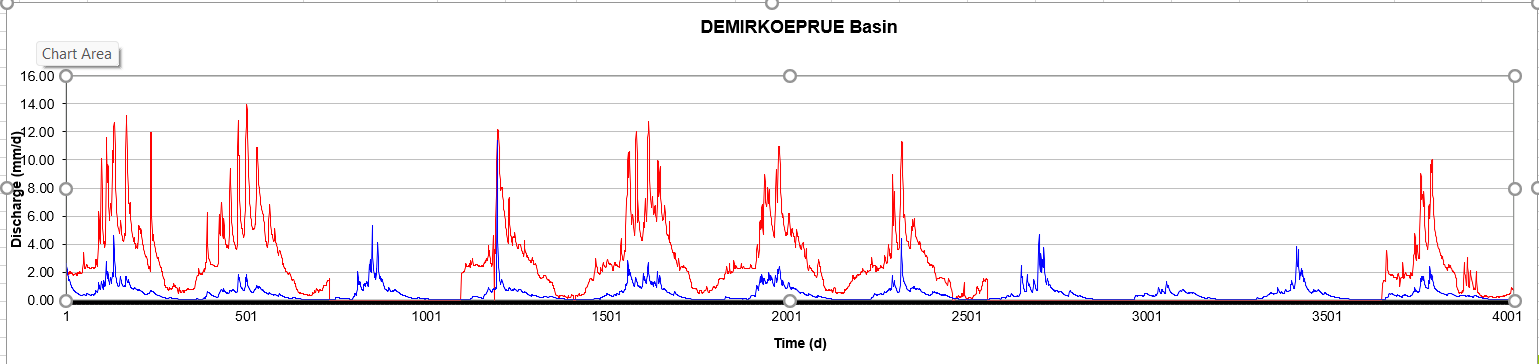
\includegraphics[width=0.8\textwidth]{image_2024-05-21_221346233.png}
    \caption{Comparison of observed and simulated discharge}
    \label{fig:discharge_comparison}
\end{figure}

\begin{table}[h]
    \centering
    \caption{Model Performance Metrics}
    \label{tab:performance_metrics}
    \begin{tabular}{l c}
        \toprule
        Metric & Value \\
        \midrule
        Nash-Sutcliffe Efficiency & -0.30 \\
        \bottomrule
    \end{tabular}
\end{table}


\section{Discussion}
The calibrated model showed a poor fit with the observed data, as indicated by the low Nash-Sutcliffe efficiency value. This discrepancy is primarily due to the absence of input data for average temperature, which is crucial for accurately modeling evapotranspiration and snowmelt processes. 

The lack of temperature data means that the model cannot account for periods of snowfall and subsequent snowmelt, which are significant factors in the hydrology of the Orontes River Basin. These limitations suggest that further refinement of the model parameters and the inclusion of comprehensive temperature data are necessary to improve model performance.

\section{Conclusion}
This assignment demonstrated the application of hydrological modeling techniques to the Orontes River Basin. The process involved setting up the HBV model with available precipitation and potential evapotranspiration data. However, the absence of average temperature data significantly impacted the model's performance, leading to a poor fit between observed and simulated discharge, as indicated by the Nash-Sutcliffe efficiency.

The model's inability to account for snowfall and snowmelt processes due to missing temperature data highlights the importance of comprehensive meteorological inputs in hydrological modeling. Future work should focus on obtaining and incorporating average temperature data to improve the accuracy of the model. Further refinement of model parameters, along with enhanced data inputs, is essential for better simulation of the hydrological processes in the Orontes River Basin.

% References
\bibliographystyle{plainnat}
\bibliography{References}
\cite{booij2005impact}
\end{document}
